\documentclass[11pt]{article}

\usepackage{graphicx} % Required for inserting images
\usepackage{biblatex}
\usepackage{indentfirst}
\usepackage[margin=1in]{geometry}
\usepackage{amsmath, amssymb}
\usepackage{float}
\usepackage{hyperref}
\setlength{\baselineskip}{1.0pt}
\setlength{\parindent}{0.5in}


\addbibresource{references.bib}

\title{Preliminary Design Review}
\author{Akhil Boyapati, Warren Cooper, Kyle Hoekema, Jennifer Ren}
\date{November 21, 2026}

\begin{document}

\maketitle

\section{Introduction}
Quadcopters are unmanned aerial vehicles (UAVs) that maneuver using four individual rotors. These rotors enable both translational and rotational movement, allowing for six degrees of freedom for the quadcopter. The purpose of this project is to create a dynamical model of a four axis symmetric drone that possesses four rotors. Within the scope of the project, there are several requirements that must be met.

\begin{enumerate}
\item The altitude of the quadcopter shall only be altered by changing the torque of the motor, which shall be individually controlled by each blade.
\item The quadcopter shall have six degrees of freedom. The quadcopter shall also account for gravity and lift generated from the rotors.
\item The quadcopter shall be able to achieve the performance goals of:
\begin{enumerate} 
\item Hover for two minutes at one meter above the ground
\item Fly in a circle with a radius of two meters, one meter above the ground, moving at one-half meters per second, for at least one minute.
\item Launch from the ground and ascend upward until it reaches one meter above the ground. Move in a straight line at one meter above the ground at an average speed of one meter per second for a total distance of five meters, hover, yaw 90 degrees to the left, once again move in a straight line for five meters, hover, and land with a speed no greater than one centimeter per second.
\end{enumerate}
\end{enumerate}

To verify the required criteria, solutions to the dynamical model must be provided using the initial conditions. Graphical visualizations must also be provided. In addition, to prove feasibility, commercial off-the-shelf components will be provided, along with justification of functionality.
\par
\vspace{0.1in}
Prior to starting the mathematics, several commercial off-the-shelf components were identified to be used as a basis for calculations. They were also selected to prove feasibility in that the quadcopter model could be made in real life.  The components include: 

    \begin{itemize}
    \item Holybro X500 V2 Drone Kit
    \item Tattu 5200mAh 4S 35C 14.8V Lipo Battery
    \item Holybro Pixhawk 6C Flight Controller
    \item Holybro PM02D Power Module
    \item Holybro DroneCAN M8N GPS
    \end{itemize}
    \par
The following Bill of Materials provides costs and links to all of the parts:

\begin{center}
\begin{tabular}{ |c|c|c| } 
 \hline
 Item Name & Cost & Link\\ 
 
 \hline
 Drone Kit (Includes Frame, motors, ESCs, PDB, props)  & \$329.00 & \href{https://holybro.com/products/x500-v2-kits?variant=42541212041405}{Kit} \\
 
 Battery & \$62.99 & \href{https://genstattu.com/tattu-5200mah-14-8v-35c-4s1p-lipo-battery-pack-with-xt60-plug.html}{Battery} \\
 
 Flight controller & \$199.00 & \href{https://holybro.com/products/pixhawk-6c?variant=42420293501117}{Flight controller} \\
 
 Power module & \$24.99 & \href{https://holybro.com/products/pm02d-power-module }{Power module} \\
 
 GPS & \$29.99 & \href{https://holybro.com/products/dronecan-m8n-gps }{GPS}\\
 
 \hline
\end{tabular}
\end{center}

Parts from the drone kit were subsequently analyzed to determine the specifications of the motor, the ESP, and the propeller. The battery, flight controller, power module, and GPS were also analyzed. From these analyses, the voltage, current, and weight, and sizing were determined for each individual component, and subsequently added up to give the constraints of:
\begin{itemize}
    \item Total Mass: 1551.8 grams
%     \item Total Voltage Draw:
%     \item Total
\end{itemize}

\newpage
\section{Mathematical Description}
The quadcopter was modeled as one rigid body with four rotors. Newton's second law was used for the motion of the center of mass (CoM) and Euler's equations for the rotation. An equation for the speed of each rotor was added too, as well as one for the battery charge - which gives 17 states in total. The only inputs are the four motor torques, which matches ER2.
\subsection{Frames and Rotor Layout}
The world frame is fixed to the ground with $z$ pointing up, so $z$ is the altitude. The body frame is attached to the CoM with $x$ pointing to the nose, $y$ to the left and $z$ up. The CoM is assumed to be at the center of the four rotors.

For the attitude, the Z-Y-X (3-2-1) Tait-Bryan angles are used \cite[p.~39]{ae352ch6}: yaw $\psi$, pitch $\theta$, and roll $\phi$, respectively. The rotation matrix from the body frame to the world frame is
\begin{equation}
R = R_z(\psi)R_y(\theta)R_x(\phi) =
\begin{bmatrix}
c_\psi c_\theta & c_\psi s_\theta s_\phi - s_\psi c_\phi & c_\psi s_\theta c_\phi + s_\psi s_\phi\\
s_\psi c_\theta & s_\psi s_\theta s_\phi + c_\psi c_\phi & s_\psi s_\theta c_\phi - c_\psi s_\phi\\
-s_\theta & c_\theta s_\phi & c_\theta c_\phi
\end{bmatrix},
\label{eq:R}
\end{equation}
where $c$ and $s$ stand for $\cos$ and $\sin$.

The rotors are in an X layout and numbered like PX4 (Figure~\ref{fig:layout}): 1 front right, 2 rear left, 3 front left, 4 rear right. With arm length $L$ and $a = L/\sqrt{2}$, rotor $i$ sits at $(x_i, y_i) = (a,-a), (-a,a), (a,a), (-a,-a)$ for $i = 1,\dots,4$. Rotors 1 and 2 spin counterclockwise (seen from above) and rotors 3 and 4 spin clockwise. We write this as $s_i = +1$ for $i=1,2$ and $s_i = -1$ for $i=3,4$. At hover, the reaction torques of the counterclockwise pair (1, 2) and the clockwise pair (3, 4) cancel when all four rotors run at the same speed.

\begin{figure}[H]
    \centering
    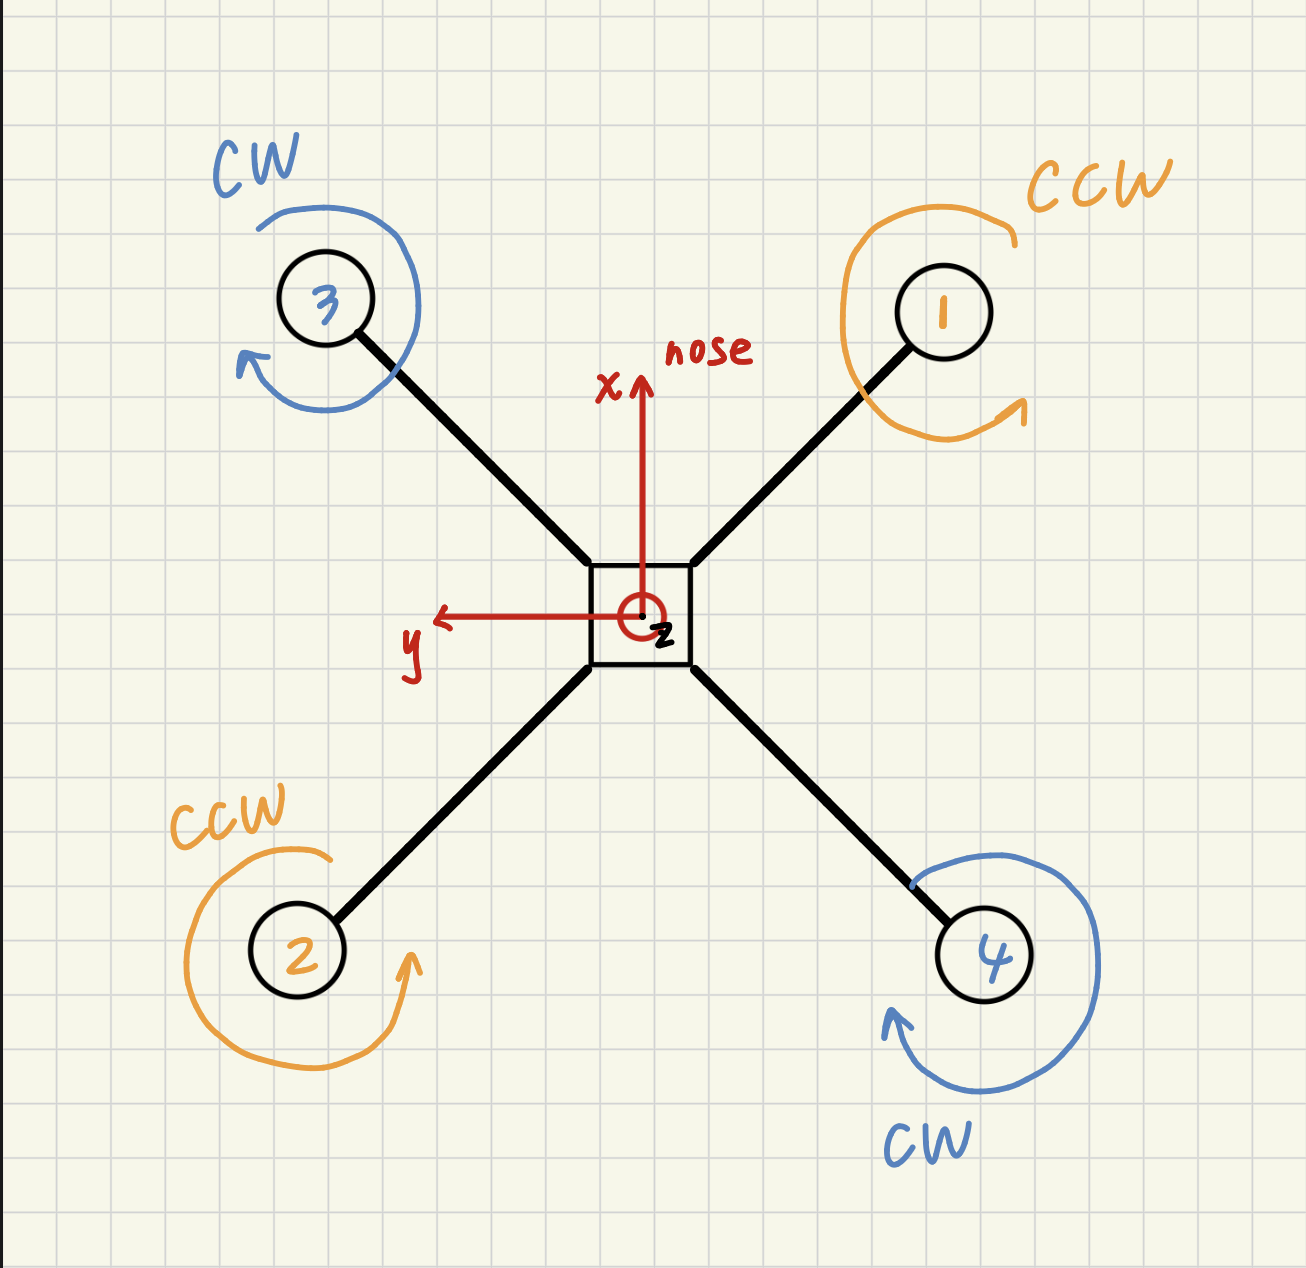
\includegraphics[width=0.5\textwidth]{layout_sketch.png}
    \caption{Top view of the drone with body axes, rotor numbers and spin directions.}
    \label{fig:layout}
\end{figure}

\subsection{States and Inputs}
The state vector is
\begin{equation}
\mathbf{x} = \big[\, \underbrace{x,\ y,\ z,\ \dot x,\ \dot y,\ \dot z}_{\text{CoM}},\ \underbrace{\phi,\ \theta,\ \psi,\ p,\ q,\ r}_{\text{attitude}},\ \underbrace{\Omega_1,\ \Omega_2,\ \Omega_3,\ \Omega_4}_{\text{rotors}},\ Q_b \,\big]^T .
\end{equation}
The first six are the CoM position and velocity in the world frame. Then come the Euler angles and the body angular velocity $\boldsymbol{\omega} = [p, q, r]^T$. These twelve states are the 6 degrees of freedom (ER1). $\Omega_i$ is the spin rate of rotor $i$ in rad/s and $Q_b$ is the charge taken from the battery. The inputs are the motor torques $\tau_1, \dots, \tau_4$.

\subsection{Rotor Model}
Each rotor makes a thrust $T_i$ along the body $z$ axis and a drag torque $Q_i$ that resists its spin:
\begin{equation}
T_i = k_T\,\Omega_i^2, \qquad Q_i = k_Q\,\Omega_i^2.
\end{equation}
To get $k_T$ and $k_Q$ we use the standard static propeller coefficients \cite{deters2008static}, which are defined with the rotation rate $n$ in rev/s as
\begin{equation}
C_T = \frac{T}{\rho n^2 D^4}, \qquad C_P = \frac{P}{\rho n^3 D^5},
\end{equation}
where $\rho$ is the air density, $D$ is the propeller diameter and $P$ is the shaft power. Plugging in $n = \Omega/2\pi$ and $P = Q\,\Omega$ gives
\begin{equation}
k_T = \frac{C_T \rho D^4}{4\pi^2}, \qquad k_Q = \frac{C_P \rho D^5}{8\pi^3}.
\end{equation}
The motor torque speeds the rotor up, and the drag torque and friction slow it down:
\begin{equation}
J_r\,\dot{\Omega}_i = \tau_i - k_Q\,\Omega_i^2 - \tau_f,
\label{eq:rotor}
\end{equation}
where $J_r$ is the rotor inertia, $\dot\Omega_i$ is its angular acceleration, and $\tau_f = I_0/K_v$ is the friction torque from the motor's no-load current $I_0$ and speed constant $K_v$ (in SI units). This is Newton's second law for rotation about the rotor axis, and it is how the motor torque changes the rotor speed, which is what ER2 asks for.

\subsection{Translational Motion}
The forces are the total thrust, gravity and air drag. The thrust points along the body $z$ axis, so we rotate it into the world frame with the rotation matrix $R$ from Equation~\eqref{eq:R}. Newton's second law gives
\begin{equation}
m\,\ddot{\mathbf{r}} = R\begin{bmatrix}0\\0\\ T\end{bmatrix} - m g\,\mathbf{e}_z - \tfrac{1}{2}\rho\, C_dA\,\lVert\dot{\mathbf{r}}\rVert\,\dot{\mathbf{r}},
\qquad T = \sum_{i=1}^{4} T_i,
\label{eq:trans}
\end{equation}
where $\mathbf{r} = [x,y,z]^T$, $m$ is the mass and $C_dA$ is the drag area. Only the last column of $R$ matters here, so for example the vertical equation is $m\ddot z = T\cos\theta\cos\phi - mg - D_z$, where $D_z$ is the vertical part of the drag. This shows that the drone has to tilt to move sideways, so the position and attitude are coupled. For takeoff and landing we also add the ground as a constraint $z \geq 0$: when the drone touches the ground, its downward velocity and rotation are set to zero, so it rests on its landing gear.

\subsection{Rotational Motion}
The Euler angle rates come from the body rates through
\begin{equation}
\begin{bmatrix}\dot\phi\\ \dot\theta\\ \dot\psi\end{bmatrix} =
\begin{bmatrix}
1 & s_\phi \tan\theta & c_\phi \tan\theta\\
0 & c_\phi & -s_\phi\\
0 & s_\phi/c_\theta & c_\phi/c_\theta
\end{bmatrix}
\begin{bmatrix}p\\ q\\ r\end{bmatrix}.
\end{equation}
This breaks down at $\theta = \pm 90^\circ$, but our controller keeps the tilt under $35^\circ$.
The body rates follow Euler's equations \cite[p.~34]{ae352ch6}:
\begin{equation}
I\,\dot{\boldsymbol{\omega}} + \boldsymbol{\omega}\times(I\boldsymbol{\omega}) = \mathbf{M}_T + \mathbf{M}_R - \boldsymbol{\omega}\times\mathbf{h}_r,
\label{eq:euler}
\end{equation}
where $I = \mathrm{diag}(I_{xx}, I_{yy}, I_{zz})$ is the inertia tensor. It is diagonal because the drone is symmetric. We estimated it by treating the motors as point masses at the arm tips, the arms as thin rods and the hub, battery and landing gear as boxes. 
\newline
The three moments on the right side: The first moment comes from the thrust. Each thrust acts at its rotor position, so the thrust moment is $\mathbf{M}_T = \sum \mathbf{r}_i \times [0,0,T_i]^T$, which gives
\begin{equation}
\mathbf{M}_T = \begin{bmatrix} a\,(-T_1 + T_2 + T_3 - T_4)\\ a\,(-T_1 + T_2 - T_3 + T_4)\\ 0 \end{bmatrix}.
\end{equation}
This moment controls roll and pitch. More thrust on the left rotors (2, 3) rolls the drone to the right, and more thrust on the rear rotors (2, 4) pitches the nose down. The thrust cannot create a yaw moment, since all thrusts are vertical.\\
The second moment is the reaction torque from the motors. Each motor pushes back on the frame with $-\tau_i$ about its spin axis, so
\begin{equation}
M_{R,z} = -\tau_1 - \tau_2 + \tau_3 + \tau_4 .
\end{equation}
At constant rotor speed this equals the drag torques $k_Q\Omega_i^2 + \tau_f$. In our model, the yaw moment comes only from these reaction torques. To yaw left, the mixer speeds up the clockwise rotors (3, 4) and slows down the counterclockwise ones (1, 2), while keeping the total thrust at the requested value.\\
The last term is the gyroscopic moment. The spinning rotors have angular momentum $\mathbf{h}_r = J_r \sum s_i\Omega_i\,\mathbf{e}_z$. It is zero at hover, when all rotors spin at the same speed, and only adds a small coupling during maneuvers.

\subsection{Battery Model}
To check ER3 we track the battery charge. Each motor draws a current $|\tau_i|/K_t$ with $K_t = 1/K_v$, and its power is that current times the back EMF $\Omega_i/K_v$ plus the resistive loss. The battery current $I_b$ is found from the total power (motors through the ESCs plus the avionics) and the battery voltage, which we model as $4(3.5 + 0.7\,\mathrm{SOC})$ volts, where SOC is the state of charge (1 when full), minus the drop across the internal resistance. Then
\begin{equation}
\dot Q_b = I_b, \qquad \mathrm{SOC} = 1 - Q_b/C,
\end{equation}
where $C$ is the battery capacity. We count ER3 as met if the state of charge stays above 20\%. 

\subsection{Hover and Control}
At hover all derivatives are zero and the drone is level, so Equations \eqref{eq:trans} and \eqref{eq:rotor} give
\begin{equation}
\Omega_h = \sqrt{\frac{mg}{4k_T}}, \qquad \tau_h = k_Q\Omega_h^2 + \tau_f .
\end{equation}
For our drone this is $\Omega_h = 518$ rad/s (4942 rpm) and $\tau_h = 71$ mN\,m per motor. This equilibrium is unstable, since any small tilt makes the drone drift away, so we need a feedback controller. Ours has three layers. A position loop (PID) finds the thrust direction needed to follow the path. An attitude loop (PD) finds the moments needed to reach that tilt. A mixer turns the thrust and moments into four rotor speeds, and a speed loop (like the ESC) sets the motor torques to reach them.

\subsection{Parameters}

Table~\ref{tab:params} lists the main parameters. They come from the Holybro X500 V2 kit and the Tattu 4S 5200 mAh battery. Values marked with $^*$ are our own estimates and still need to be checked against propeller test data.
\begin{table}[htbp]
\centering
\caption{Main model parameters.}
\label{tab:params}
\small
\begin{tabular}{l c l}
\hline
Parameter & Symbol & Value \\
\hline
Mass & $m$ & 1.552 kg \\
Arm length & $L$ & 0.25 m \\
Moments of inertia & $I_{xx}, I_{yy}, I_{zz}$ & 0.0217, 0.0211, 0.0325 kg\,m$^2$ \\
Propeller diameter & $D$ & 0.254 m \\
Propeller coefficients & $C_T$, $C_P$ & 0.11$^*$, 0.045$^*$ \\
Thrust constant & $k_T$ & $1.42\times10^{-5}$ N\,s$^2$ \\
Torque constant & $k_Q$ & $2.35\times10^{-7}$ N\,m\,s$^2$ \\
Rotor inertia & $J_r$ & $7.5\times10^{-5}$ kg\,m$^2$ $^*$ \\
Motor speed constant & $K_v$ & 920 rpm/V \\
Motor currents (no-load, max) & $I_0$, $I_{max}$ & 0.8 A, 17 A \\
Battery & & 4S, 5.2 Ah \\
Drag area & $C_dA$ & 0.06 m$^2$ $^*$ \\
\hline
\end{tabular}
\end{table}

\newpage
\section{Results}
\par Results of mathematics

\newpage
\section{Contributions}
\par \textbf{Akhil Boyapati - Software and Implementation lead}
% \par Akhil was responsible for creating the software needed to simulate the digital twin. (Add whatever else as time goes on)
\vspace{0.1in}
\par \textbf{Warren Cooper - Procurement Specialist and Quality Control Engineer}
\par Warren was responsible for researching physical materials that would demonstrate feasibility of the quadcopter and making sure all requirements for the report were met. %(Add whatever else as time goes on)
\vspace{0.1in}
\par \textbf{Kyle Hoekema - Lead Engineer}
\par Kyle was responsible for drafting up the report, coordinating, ensure adherence to schedule. %(Add whatever else as time goes on)
\vspace{0.1in}
\par \textbf{Jennifer Ren - Design Engineer}
\par Jennifer was responsible for the engineering design and visualization %(Add whatever else as time goes on)


\newpage
\printbibliography
\end{document}
